% Latencias p50/p95 reales por agente extraídas de logs/app.log
% (eventos con status="ok"). Excluye admin_orchestrator porque su
% p95 (36 s, n=7) está dominado por una arranque en frío del LLM y
% distorsionaría la escala.
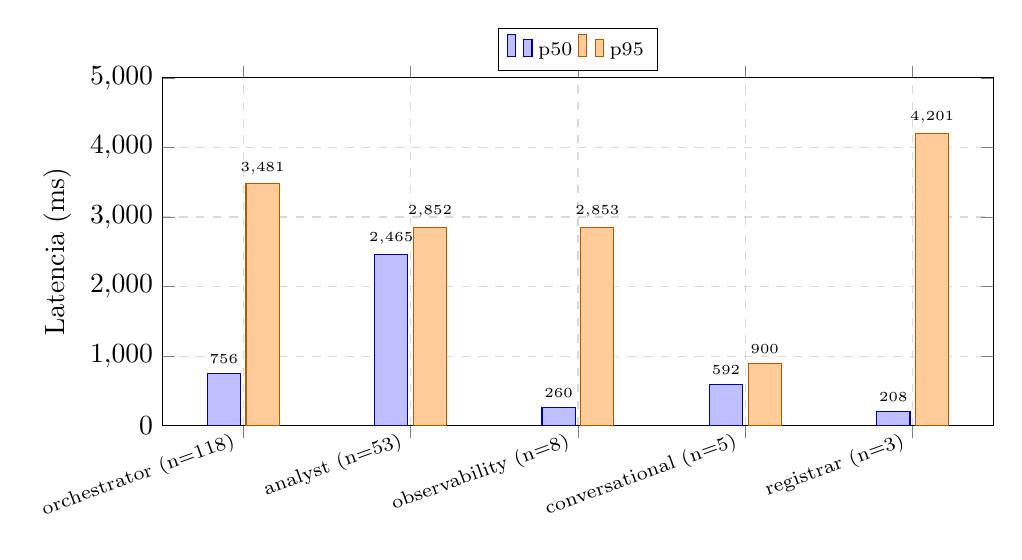
\begin{tikzpicture}
\begin{axis}[
    width=\linewidth, height=6cm,
    ybar,
    bar width=12pt,
    ylabel={Latencia (ms)},
    ymin=0, ymax=5000,
    ytick={0,1000,2000,3000,4000,5000},
    symbolic x coords={orchestrator (n=118), analyst (n=53),
                       observability (n=8), conversational (n=5),
                       registrar (n=3)},
    xtick=data,
    x tick label style={rotate=20,anchor=east,font=\scriptsize},
    legend style={at={(0.5,1.02)},anchor=south,legend columns=2,font=\scriptsize},
    nodes near coords,
    nodes near coords style={font=\tiny},
    every node near coord/.append style={/pgf/number format/.cd, fixed, precision=0},
    grid=major,
    grid style={dashed, gray!30},
    enlarge x limits=0.12,
]
\addplot[fill=blue!25,draw=blue!60!black] coordinates {
  (orchestrator (n=118),756)
  (analyst (n=53),2465)
  (observability (n=8),260)
  (conversational (n=5),592)
  (registrar (n=3),208)
};
\addplot[fill=orange!40,draw=orange!70!black] coordinates {
  (orchestrator (n=118),3481)
  (analyst (n=53),2852)
  (observability (n=8),2853)
  (conversational (n=5),900)
  (registrar (n=3),4201)
};
\legend{p50, p95}
\end{axis}
\end{tikzpicture}
